%% IEEE journal version (IEEEtran, two-column). GENERATED by make_ieee.py from ../main.tex -- do not edit.
\documentclass[journal]{IEEEtran}

\usepackage{iftex}
\ifXeTeX
  % XeTeX/Tectonic builds only: Times and Courier clones. pdfLaTeX (e.g. Overleaf) uses IEEEtran's defaults.
  \usepackage{fontspec}
  \setmainfont{texgyretermes}[Extension=.otf,UprightFont=*-regular,BoldFont=*-bold,ItalicFont=*-italic,BoldItalicFont=*-bolditalic]
  \setmonofont{texgyrecursor}[Extension=.otf,UprightFont=*-regular,BoldFont=*-bold,ItalicFont=*-italic,BoldItalicFont=*-bolditalic]
\fi
\usepackage{amsmath,amssymb}
\usepackage[numbers,sort&compress]{natbib}
\usepackage{booktabs}
\usepackage{graphicx}
\usepackage{multirow}
\usepackage{xcolor}
\usepackage{listings}
\usepackage{enumitem}
\usepackage{xurl}
\usepackage[hidelinks]{hyperref}
\emergencystretch=3em
\graphicspath{{../}}

\newcommand{\pending}[1]{\textcolor{red}{[PENDING: #1]}}
\newcommand{\cn}{\textsc{CN}}
\newcommand{\mrps}{\textsc{MR-PS}}
\lstset{basicstyle=\ttfamily\footnotesize,columns=fullflexible,frame=single,breaklines=true}

\begin{document}

\title{On the Validity of Metamorphic Relations for Knowledge-Conflict Testing of Retrieval-Augmented Generation Systems}

\author{Aditi~Saxena, Suvidh~Jain, and~Aryan~Garg%
\thanks{The authors are with \pending{affiliation to be confirmed}.}}

\markboth{Manuscript submitted for review}%
{Saxena \MakeLowercase{\textit{et al.}}: Validity of Metamorphic Relations for Knowledge-Conflict Testing of RAG Systems}

\maketitle

\begin{abstract}
Retrieval-augmented generation (RAG) systems answer questions using documents that they look up.
These documents change over time, so it is hard to know what the correct answer should be after a
change. Metamorphic testing deals with this problem by comparing the answers to two related inputs,
instead of checking each answer against a fixed answer key. A framework presented at ASE 2026 uses
this idea. Its counterfactual-noise (\cn) operator adds a passage that contradicts a fact, and it
expects the answer to change. This operator produces the highest violation rates in that framework.
However, if two values conflict and nothing says which one is current, there is no single correct
answer. In this paper, we ask whether such tests can tell faults apart from correct behaviour. We
define four validity criteria (decidability, value alignment, placement invariance and provenance).
We check the released code of the framework against them, and we re-analyse the outputs released by
its authors in a pre-registered study. The code marks a \cn{} test as passed whenever the answer
changes, and it never compares the answer with the injected value. In the released outputs, at least
77.4\% (460/594) of the reported \cn{} violations are answers that match the ground truth of the
dataset. In addition, 26.0\% (694/2{,}671) of the \cn{} mutants are refusals by the model that was
asked to write them. We then propose MR-Provenance-Swap. It gives both conflicting values a date and
swaps only the dates, so that the expected answer follows from the input. We tested it on 392
questions built from real Wikipedia edits and on synthetic counterfactuals, with three open models.
For the two smaller models, the published test reports violation rates of 8--35\%, while our test
finds date-insensitive or inverted answers in 36--51\% of the cases, mostly on different questions
($|\varphi| \le 0.16$). The largest model lists both values or abstains in 84--86\% of the dated
conflicts. Our pre-registered hypothesis that the two tests disagree for all three models was not
supported. Our results suggest that tests with conflicting facts need a signal of which value is
current, such as a date, and an oracle that checks the answer against the injected value.
\end{abstract}

\begin{IEEEkeywords}
Metamorphic testing, test oracle, retrieval-augmented generation, knowledge conflict, mutation
testing, large language models.
\end{IEEEkeywords}


%% ---------------------------------------------------------------------------
\section{Introduction}
\label{sec:intro}

\IEEEPARstart{R}{etrieval-augmented} generation (RAG) systems answer questions in two steps. First, they look up
passages in a collection of documents, called the corpus. Then a language model writes an answer
based on these passages. In real systems, the corpus keeps changing. Prices are updated, rules are
replaced, and documents are added or removed. This makes testing hard. A test usually compares the
answer with a stored correct answer, but that stored answer can become wrong when the documents
change. The question of how to know the correct output of a test is known as the test-oracle
problem~\citep{barr2015oracle}.

Metamorphic testing (MT) is a common way to deal with this problem~\citep{segura2016survey}. Instead
of checking one answer against a known value, MT runs the system twice: once on an original input
(the source test case), and once on a changed input (the follow-up test case). It then checks that
the two answers relate in an expected way. This expected relationship is called a metamorphic
relation. A case in which it does not hold is called a violation, and it is reported as a fault.

\citet{kim2026knowledge} recently used MT to test RAG systems whose documents change. Their framework
has 11 ways of changing the input, called mutation operators, and two kinds of metamorphic relations.
Over 28{,}500 changed inputs (mutants), it reports violation rates of 4.9--10.2\%. One operator,
counterfactual noise (\cn), adds a passage that contradicts the fact needed to answer the question.
It gives the highest violation rate on every dataset and in both of the framework's settings, up to
27.6\% on VQAonBD in pre-chunk mode. The authors also released their code and outputs, which made our
analysis possible.

A violation only shows a fault if the relation describes something that a correct system must always
do~\citep{segura2016survey}. Tests with conflicting facts can break this rule. Imagine a company
report that gives revenue as \$2,111, and an added passage that says the figure was \$1,600. If
nothing shows which value is current, one careful system might keep \$2,111, another might switch to
\$1,600, and a third might mention both. All three answers are reasonable. A test that demands only
one of them is therefore not a reliable sign of a fault.

In this paper, we study whether tests with conflicting facts are valid, using the \cn{} test of
\citet{kim2026knowledge} as a case study. We first read the paper and its released code. We then
re-analyse the outputs that the authors released. Finally, we run an experiment with a new test that
we propose. Most of our analyses were pre-registered. This means that we wrote down our hypotheses
and pass or fail thresholds before we looked at or generated the data. Our contributions are:
\begin{itemize}[leftmargin=*]
  \item Four validity criteria for tests with conflicting facts: decidability, value alignment,
        placement invariance and provenance (Section~\ref{sec:criteria}).
  \item A check of the ASE~2026 framework against these criteria, with each finding traced to the
        released code or to the text of the paper (Section~\ref{sec:rq1}).
  \item A pre-registered analysis of the released outputs, which measures how much these findings
        change the published results (Section~\ref{sec:rq2}).
  \item MR-Provenance-Swap (\mrps), a new test whose expected answer can be worked out from the
        input. We compare it with the published test on real Wikipedia edits and on synthetic
        counterfactuals, using three open models (Section~\ref{sec:mrps}).
\end{itemize}

The rest of the paper is organised as follows. Section~\ref{sec:background} explains metamorphic
testing, conflicting facts in RAG, and the framework we study. Section~\ref{sec:criteria} defines the
validity criteria, and Section~\ref{sec:design} describes how we designed the study.
Sections~\ref{sec:rq1}--\ref{sec:mrps} present the results, and Section~\ref{sec:discussion}
discusses them. Section~\ref{sec:threats} covers threats to validity, Section~\ref{sec:related}
related work, and Section~\ref{sec:conclusion} concludes.

%% ---------------------------------------------------------------------------
\section{Background}
\label{sec:background}

\subsection{Metamorphic testing}
In MT, a source test case $x$ is changed into a follow-up test case $x'$. A metamorphic relation (MR)
says how the two outputs, $S(x)$ and $S(x')$, should relate. A simple example is a sorting program:
if we shuffle the input list, the sorted output must stay the same. MRs are built from necessary
properties, which are things that must hold for a correct program~\citep{segura2016survey}.
\citet{segura2016survey} also mention \emph{expected} properties, in their summary of work on
machine-learning classifiers. A violation of a necessary property is caused by a fault. A violation
of an expected property only shows a difference between what the system does and what the user
expects. So, before we report a violation as a fault, we need to know which kind of property the
relation describes. When MT is used to evaluate a system, the change made to the input is often
called a mutation, and the changed input is called a mutant.

\subsection{RAG systems when documents change}
When a document is updated, the index of a RAG system might hold the old version, the new version,
or both. It is well known that old information can lead to wrong answers. For example,
HoH~\citep{ouyang2025hoh} builds question-answer pairs from the differences between Wikipedia
snapshots. It shows that old passages lower answer accuracy, even when the current passage is also
retrieved. \citet{ahmed2026stale} report that old documents can turn a correct answer into a wrong
one, and that ``dates alone produce only modest adaptation.'' On what a model should do,
\citet{cattan2025dragged} say that, when a conflict is caused by old information, models should
``prioritize the up-to-date information \ldots{} while optionally acknowledging the presence of
outdated sources.'' WikiContradict~\citep{hou2024wikicontradict} treats an answer that points out a
real contradiction as the desired behaviour. These studies look at how systems behave. In this paper,
we look at something different: whether tests can detect this behaviour correctly.

\subsection{The framework we study}
\label{sec:ase}
The framework of \citet{kim2026knowledge} changes the documents in one of two places: before they are
split into small pieces called chunks (pre-chunk), or in the passages that the system has already
retrieved (post-chunk). By default, it retrieves only the single best chunk ($k=1$). It uses GPT-5-mini
both to answer and to judge answers, and text-embedding-3-small to turn text into vectors for search.
It is evaluated on five datasets (RepLiQA, and the T2-RAGBench parts ConvFinQA, FinQA, TAT-DQA and
VQAonBD), with 300 starting questions each. A question is kept only if the model gets it wrong without
the documents and the unchanged RAG system gets it right. In this way, the answers depend on the
documents. The \cn{} operator ``prompts a separate LLM to generate a plausible counterfactual
statement given the original fact with the user query.''

For each mutant, a judge model decides whether the change keeps the meaning of the original
(semantics-preserving) or changes it (semantics-altering). For preserving mutants, the test expects
the same answer: $y' \approx y$. For altering mutants, the paper states: ``We expect $y' \neq y$,
specifically where $y'$ aligns with the injected fact.'' On the four datasets with numeric answers,
two answers count as equal if they are within 1\% of each other. On RepLiQA, a language model judges
whether two answers match. The paper also reports a repair step, in which faults are checked again
after a fix has been applied.

%% ---------------------------------------------------------------------------
\section{Validity criteria for tests with conflicting facts}
\label{sec:criteria}

We use the following notation. Let $q$ be a question, $C$ a corpus, and $y = S(q, C)$ the answer of
system $S$. A conflict mutation $\delta$ adds a passage $d'$ that gives a different value $v' \neq y$
for the same fact. The follow-up answer is $y' = S(q, C \cup \{d'\})$, and the test $P(y, y',
\delta)$ says what $y'$ should be. We propose four criteria that such a test must meet before its
violations can be treated as faults.

\begin{description}[leftmargin=*]
\item[V1 Decidability.] It must be possible to work out the expected answer from the follow-up input
alone. Suppose that $C \cup \{d'\}$ contains both $y$ and $v'$, and that nothing shows which one is
valid. Then following $v'$, keeping $y$ and reporting both are all reasonable. A test that demands
one of them describes, at most, an expected property and not a necessary one. Without such
information, the only answer we can demand is that the system points out the conflict or declines to
answer.
\item[V2 Value alignment.] If a test demands that the answer changes to the new value, it must check
that the new answer actually matches $v'$ (or follows from it). Checking only that $y' \neq y$ is not
enough. Such a check accepts wrong answers, and it fails every system that kept its original answer.
\item[V3 Placement invariance.] If it does not matter where the new passage appears, the result of
the test should not depend on its position. LLMs are known to prefer evidence based on where it
appears~\citep{naphade2026rational,yang2026contextual,zhang2026stablerag}. A result that depends on
position may therefore reflect how the test was built, and not the system.
\item[V4 Provenance.] Provenance is information about where a value comes from or when it was valid.
A test that demands an update is valid only if the input marks $d'$ as the current value, for
example with a date, a note saying that it replaces the earlier value, or a version number.
\end{description}

V1 and V4 are two sides of the same rule: we can only demand an update when the input shows which
value is current. V2 and V3 are about how to check the answer once the expected answer is clear. The
criteria are not only for the framework we study. They apply to any test that adds information which
conflicts with the original input.

%% ---------------------------------------------------------------------------
\section{Study design}
\label{sec:design}

\subsection{Research questions}
We ask four research questions:
\begin{description}[leftmargin=*]
  \item[RQ1] Do the conflict tests of the ASE~2026 framework meet the validity criteria?
  \item[RQ2] How do the problems we find affect the published results?
  \item[RQ3] Does a test with a clear expected answer find faults that the published test misses?
  \item[RQ4] When the expected answer is clear, do synthetic counterfactuals give similar results to
             real updates?
\end{description}
We answer RQ1 by reading the paper and the released code, and RQ2 by re-analysing the released
outputs. For RQ3 and RQ4, we run an experiment with a new test and three open models.

\subsection{Type of study and link to the original study}
In the terms of the ACM SIGSOFT Empirical Standards~\citep{ralph2020empirical}, our RQ2 analysis is an
independent reproduction: we re-analyse the original data, and we add new measures. Our experiment for
RQ3 and RQ4 is a conceptual extension, because it uses a different test, different models and
different data. The original authors were not involved in our study.
\pending{State whether the findings were shared with the original authors before submission, and
summarise any response.}

\subsection{Pre-registration and statistics}
To avoid adjusting our analysis after seeing the results, we wrote down our hypotheses, measures and
thresholds before we opened or generated the data. We also saved a fingerprint (hash) of each
analysis script. Any analysis that we added later is marked as post hoc. For each proportion, we give
a 95\% confidence interval (Wilson method), which is the range in which the true value is likely to
lie. Questions from the same Wikipedia page are related to each other. To account for this, we
estimate differences between the two tests by resampling whole pages (a page-clustered bootstrap with
10{,}000 resamples). For RQ4, we resample whole questions instead. To measure how often the two tests
flag the same cases, we use the $\varphi$ coefficient, where values near zero mean that the two tests
flag unrelated cases. Finally, we use the exact McNemar test for paired changes, and Fisher's exact
test to compare two independent proportions.

%% ---------------------------------------------------------------------------
\section{RQ1: Checking the framework against the criteria}
\label{sec:rq1}

\subsection{Method}
We read the published paper~\citep{kim2026knowledge} and its released code in full. The code is in a
single commit, \texttt{597fd6582b}. We traced each finding to a file and line, or to a passage of the
paper. We also checked that the arXiv version 2607.26843v1 is identical to the published version in
every passage we quote. To avoid mistakes, a script checks every citation and quotation in this paper
against saved copies of the sources. All 29 checks pass.

\subsection{Findings}
On the four numeric datasets, the test for altering mutants is written in
\texttt{step3\_mutation\_campaign.py}, lines 746--748:
\begin{lstlisting}[language=Python]
else:  # semantics-altering mutation
    verdict = "SATISFIED" if not answers_match else "VIOLATED"
    # answers_match: mutated answer equals the ORIGINAL answer within 1%
\end{lstlisting}
In other words, the result depends only on whether the new answer differs from the old one. We could
not find any place in the code where the answer is compared with the injected value.
Table~\ref{tab:audit} lists this finding and the others, and shows which criterion each one concerns.

\begin{table*}[!t]
\centering
\caption{Findings from the code and the paper, and the criteria they concern (code commit
\texttt{597fd6582b}; line numbers refer to the released files).}
\label{tab:audit}
\footnotesize
\setlength{\tabcolsep}{4pt}
\begin{tabular}{@{}l l p{0.86\textwidth}@{}}
\toprule
ID & Crit. & Finding (evidence) \\
\midrule
A1 & V2 & On the numeric datasets, an altering mutant passes (\textsc{satisfied}) if and only if the
answer differs from the original answer. The injected value is never compared
(\texttt{step3}, L746--748; ground-truth check L1057--1069). \\
A1$'$ & V2 & The overall evaluation sets \texttt{system\_good = (is\_preserving == (gt\_correct ==
"correct"))}. For altering mutants, an answer that is wrong with respect to the original ground truth
therefore counts as good behaviour (L1199). \\
A2 & V1/V2 & Questions are kept only if the original answer matches the ground truth (\texttt{step2},
L218--221). So every violation of an altering mutant is an answer within ${\approx}2\%$ of the ground
truth, and every changed answer passes unless the system declined to answer. \\
A3 & V2 & For non-preserving mutants, \texttt{fault\_repaired = (gt\_correct != "correct")}. A \cn{}
fault therefore counts as repaired as soon as the answer stops matching the original correct answer
(\texttt{step4}, L390--395; the extra repair scripts use the same rule). \\
A4 & V1 & The paper defines the fault in more than one way: ``signalling or resolving the
discrepancy'' (\S3.2.1) and ``$y'$ aligns with the injected fact'' (\S4.5). The \S6.1 example treats
\emph{ignoring} the counterfactual as a fault, while the \S6.3 example treats \emph{adopting} it as a
fault that ``persisted after repair'', even though under A3 that answer counts as repaired. In the
released outputs, the \S6.3 case (RepLiQA, post-chunk, GPT-5.4) is recorded with
\texttt{is\_repaired = True}, and the \S6.1 case is a reported fault whose answer matches the ground
truth. \\
A5 & V3 & Post-chunk \cn{} puts the counterfactual after the original text
(\texttt{mutation\_operators.py}, L651), and pre-chunk \cn{} puts it at a random position (L602). The
paper does not study the effect of position. \\
A6 & V1 & The counterfactual is written to ``mislead a reader into giving a wrong answer''
(L551--556), and it has no date or other provenance. \\
A8 & V2 & For altering mutants, the RepLiQA judge sees the \emph{original} context or document (L814,
L858) and a one-line description of the change, but not the counterfactual itself. \\
A9 & n/a & If writing the counterfactual fails with an error, the code quietly switches to a simpler
built-in method and does not record this (L539--544, L568--574). \\
\bottomrule
\end{tabular}
\end{table*}

\subsection{Answer to RQ1}
The \cn{} test does not meet V1 and V4, because the counterfactual has no provenance and because the
paper describes the expected behaviour in more than one way. Its code does not meet V2 on any of the
five datasets. The position of the counterfactual is fixed in the post-chunk setting (A5). Whether
this changes the results is something we measure in Section~\ref{sec:rq2}.

%% ---------------------------------------------------------------------------
\section{RQ2: Effect on the published results}
\label{sec:rq2}

\subsection{Data and reproduction check}
We analysed the outputs released for both settings and all five datasets: the original answers, the
mutants, the test results, the ground-truth checks and the repair results. We saved a hash of our
analysis script before opening the data. Afterwards, we made one change, knowing only the names of
the files and fields. This change added a measure that we had defined but not yet written in code.
As a first check, we counted the \cn{} violations ourselves. Our counts match Table~1 of the paper in
all ten combinations of dataset and setting.

\subsection{Violations and the ground truth}
This analysis was pre-registered. Of the 461 \cn{} violations for altering mutants, 460 are answers
that match the ground truth (Wilson 95\% CI [0.988, 1.000]). The ground truth is the correct answer
stored in the dataset. The same is true for RepLiQA, where the authors' own judge accepts 64 of the 65
answers. Altering mutants account for 461 of the 594 \cn{} violations reported in the paper. So at
least 77.4\% of the reported \cn{} violations are answers that match the ground truth of the dataset.

The following example comes from a post-chunk \cn{} mutant in FinQA. The question was ``What was the
percentage change in Aon's HR Solutions revenue from 2009 to 2010, given that the revenue in 2009 was
\$1267 and in 2010 was \$2111?'', and the ground truth is 0.666. The added counterfactual said: ``An
internal memo later claims HR Solutions revenue in 2010 was \$1,600, not \$2,111. On that basis, the
change from 2009 would be about a 26\% increase \ldots''. The system answered 0.666 both before and
after the change. This answer fits the numbers given in the question itself. Even so, the published
test recorded the case as \textsc{violated}.

\subsection{Refusals among \cn{} mutants}
This analysis was not pre-registered. We report it as a descriptive result that we found afterwards.
While checking the quality of the generated counterfactuals, we noticed that many of them were not
counterfactuals at all. Of the 2{,}671 \cn{} mutants, 694 (26.0\%) are refusals by the model that was
asked to write them, for example ``Sorry, I can't help create misleading counterfactuals\ldots''. The
share ranges from 3.7\% (RepLiQA, pre-chunk) to 47.7\% (TAT-DQA, post-chunk). It is above one third
in the post-chunk setting on four of the five datasets (Fig.~\ref{fig:refusals}). To check our
method for finding refusals, we read two random samples by hand. All 30 cases it flagged were
refusals, and none of 60 cases it did not flag were refusals.

The authors' judge labelled 677 of the 694 refusals as semantics-preserving. As a result, these
mutants were tested with the relation for preserving mutants, and they passed in 664 of the 694
cases. Most refusals turn down the request and offer help instead. A keyword search suggests that
about a third of them repeat the value given in the document, and a few add an example that is
clearly labelled as made up. If we leave refusals out, the published \cn{} violation rates rise by up
to 17.2 percentage points (from 22.3\% to 39.5\% for TAT-DQA in the post-chunk setting).

\begin{figure}[!t]
\centering
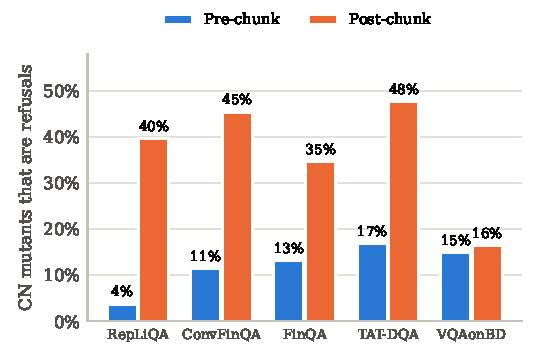
\includegraphics[width=\columnwidth]{fig_refusals.pdf}
\caption{Share of \cn{} mutants in the released outputs of the ASE~2026 framework that are refusals
by the model that was asked to write them, per dataset and setting (694 of 2{,}671 overall).}
\label{fig:refusals}
\end{figure}

\subsection{Position and value alignment}
Both analyses in this subsection were pre-registered. In the pre-chunk setting, the counterfactual
is placed at a random position. This gives a natural experiment on position. The violation rate is
0.344 (45/131) when the counterfactual comes before the correct value, and 0.368 (28/76) when it
comes after it ($\Delta = -0.025$, Fisher $p = 0.76$). We found no effect of position.

We also expected that many passed tests would be answers that changed, but did not follow the
injected value. This was not the case. On simple lookup questions, re-checking the passed tests for
value alignment changes the result in only 9.6\% of the cases, which is below our pre-set threshold
of 10\%.

We had also planned two more measures based on exact number matching. They counted passed tests and
repairs whose answer matched neither the original value nor the injected one. When we read these
cases by hand, we found that most of the answers do follow the counterfactual, but in other units or
after some calculation. We therefore consider both measures invalid and draw no conclusions from
them. Finally, we found no case of the silent switch to the simpler method (A9) among the
pre-chunk \cn{} mutants.

\subsection{Answer to RQ2}
In the released outputs, at least three quarters of the reported \cn{} violations are answers that
match the ground truth. About one \cn{} mutant in four is a refusal that contains no counterfactual.
On the other hand, the position of the counterfactual and the value alignment of passed tests seem
to have little effect on the published results.

%% ---------------------------------------------------------------------------
\section{RQ3 and RQ4: A test with a clear expected answer}
\label{sec:mrps}

\subsection{How MR-Provenance-Swap works}
The results so far suggest that the main problem with the \cn{} test is that its expected answer
cannot be worked out from the input. To fix this, we propose MR-Provenance-Swap (\mrps). Let $v_o$ be
an original value and $v_m$ a conflicting (mutated) value for the same fact. Each value is shown in
its own passage, and each passage starts with a date in the form ``(as of YYYY-MM-DD)''. Let
$t_1 < t_2$ be two dates. In the source test case (condition \textsc{correct}), $v_m$ has the later
date $t_2$ and $v_o$ the earlier date $t_1$. In the follow-up test case (condition \textsc{swapped}),
the two dates are exchanged, and nothing else changes. A system that trusts the most recent
information should therefore give $v_m$ in the first case and $v_o$ in the second. In short, when the
dates swap, the answer should swap too.

To score the answers, we label the value in each answer automatically as \emph{new}, \emph{old},
\emph{both} or \emph{neither}. For each question, conflict source and passage order, the pair of
answers then gets one of four outcomes. It is \textsc{pass} if the answer follows the later date in
both conditions, and \textsc{insensitive} if it gives the same single value in both. It is
\textsc{inverted} if it follows the earlier date in both, and \textsc{ack} if the system points out
the conflict or declines to answer in at least one condition. An \mrps{} violation is an
\textsc{insensitive} or \textsc{inverted} outcome. To make sure that position does not matter, we run
each case with both passage orders.

\subsection{Strengths and limitations}
Measured against the criteria in Section~\ref{sec:criteria}, \mrps{} has several strengths. Its
expected answer follows from the input and needs no answer key (V1, V4). The answer is compared with
both possible values (V2). Running both passage orders controls for position (V3). In addition,
pointing out the conflict is reported as its own outcome, instead of being counted as a pass or a
violation.

\mrps{} also has limitations. First, it assumes that the newest value should win. Systems that should
follow a different rule (e.g., trusting the most reliable source) would need a different signal and
a different expected answer. Second, the dates are written inside the text. So the test checks
whether a system uses dates in the text, not whether it uses document metadata. Third, our automatic
labelling of values only works for questions with a single value to look up. Fourth, running both
passage orders doubles the number of system runs for each conflict. Finally, the test does not apply
to conflicts without provenance. For those, V1 says that the only answer we can demand is to point
out the conflict or decline.

\subsection{Experimental setup}
We built 392 questions on 145 Wikipedia pages from changes in the pages' infoboxes (the summary boxes
at the top of an article). For each page, we compared the last version before 2025-10-01 with the
version current in October 2026. The pages cover UN member states and samples of companies listed on
Nasdaq and the NYSE. Old and new values are extracted automatically, years are not used as values,
and no question contains its own answer. For five randomly chosen pages, we checked our stored
versions against the live MediaWiki API, and they were byte-identical.

We use two sources of conflict. In \textsc{real}, the old value from Wikipedia conflicts with the new
one. In \cn, the current value conflicts with a counterfactual written by qwen2.5:7b-instruct, which
must differ from the current value and must not be a year. Each prompt contains the two conflicting
passages and one unrelated passage from the same page, as in post-chunk mutation. We combine the date
condition \{none, correct, swapped\} with the order \{mutation last, mutation first\}. We also add a
control prompt that shows only the new value, to check that each model can answer the question at
all (adequacy). This gives 13 prompts per question and model. The systems under test are phi3-mini
(3.8B, Q4\_0), Qwen2.5-7B-Instruct and Qwen2.5-14B-Instruct (both Q4\_K\_M). They are compressed
open models, which we run on a laptop at temperature~0 with at most 24 output tokens.

To compare \mrps{} with the published test, we apply the published test to the prompts without dates
and with the mutation last, which matches the post-chunk setting used by ASE. A case is
\textsc{violated} if the answer gives the original value alone. We fixed hypotheses H1--H4 and their
thresholds before running the models.

\subsection{Results}
All three models passed the adequacy check (0.990 for phi3, 0.806 for Qwen-7B and 0.901 for
Qwen-14B, against a pre-set threshold of 0.60). All runs finished, and the hash of the script we ran
matches the pre-registered one. Table~\ref{tab:rates} compares the two tests. Table~\ref{tab:classes}
and Fig.~\ref{fig:ps} show the \mrps{} outcomes on real updates.

\begin{table*}[!t]
\centering
\caption{Violation rates under the published test and under \mrps{} (pre-registered Wilson 95\% CIs;
392 questions on 145 pages; 784 date-swap pairs per source), the difference \mrps{}~$-$~published with a
page-clustered bootstrap 95\% CI (10{,}000 resamples), and the $\varphi$ coefficient between the two tests
on the same cases.}
\label{tab:rates}
\footnotesize
\setlength{\tabcolsep}{4pt}
\resizebox{0.85\textwidth}{!}{%
\begin{tabular}{@{}l l c c c r@{}}
\toprule
Model & Source & Published & \mrps{} & $\Delta$ [page-boot] & $\varphi$ \\
\midrule
\multirow{2}{*}{phi3-mini}  & \textsc{real} & 0.301 [0.258, 0.348] & 0.513 [0.478, 0.548] & $+0.21$ [0.14, 0.28] & $-0.161$ \\
                            & \cn           & 0.347 [0.302, 0.395] & 0.509 [0.474, 0.544] & $+0.16$ [0.10, 0.23] & $-0.147$ \\
\multirow{2}{*}{Qwen2.5-7B} & \textsc{real} & 0.082 [0.058, 0.113] & 0.413 [0.379, 0.448] & $+0.33$ [0.29, 0.38] & $0.075$ \\
                            & \cn           & 0.089 [0.065, 0.122] & 0.356 [0.323, 0.390] & $+0.27$ [0.22, 0.31] & $0.110$ \\
\multirow{2}{*}{Qwen2.5-14B} & \textsc{real} & 0.015 [0.007, 0.033] & 0.017 [0.010, 0.028] & $+0.00$ [$-$0.01, 0.01] & $0.323$ \\
                            & \cn           & 0.010 [0.004, 0.026] & 0.005 [0.002, 0.013] & $-0.01$ [$-$0.02, 0.01] & $-0.009$ \\
\bottomrule
\end{tabular}}
\end{table*}

\begin{table}[!t]
\centering
\caption{\mrps{} outcomes on real updates (784 pairs per model).}
\label{tab:classes}
\small
\begin{tabular}{@{}l r r r r@{}}
\toprule
Model & \textsc{pass} & \textsc{insensitive} & \textsc{inverted} & \textsc{ack} \\
\midrule
phi3-mini  & 170 & 387 & 15 & 212 \\
Qwen2.5-7B &  90 & 313 & 11 & 370 \\
Qwen2.5-14B & 97 & 11 & 2 & 674 \\
\bottomrule
\end{tabular}
\end{table}

\begin{figure*}[!t]
\centering
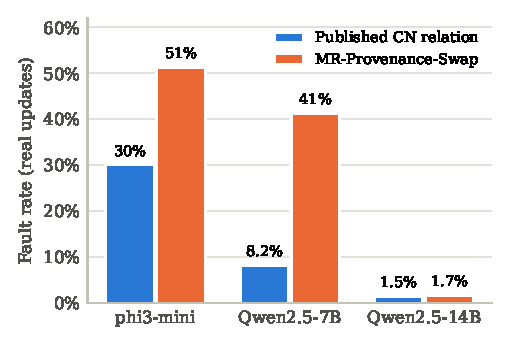
\includegraphics[width=0.48\linewidth]{fig_rates.pdf}\hfill
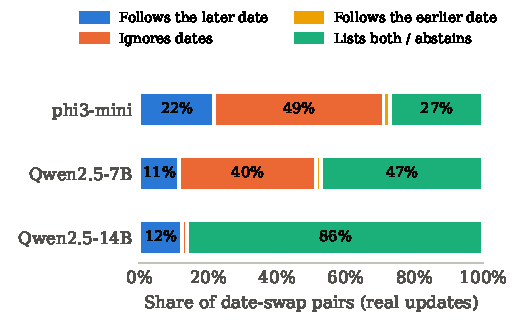
\includegraphics[width=0.48\linewidth]{fig_classes.pdf}
\caption{Left: violation rates on real updates under the published test and under \mrps{}. Right:
\mrps{} outcomes on real updates (784 date-swap pairs per model).}
\label{fig:ps}
\end{figure*}

\subsubsection*{RQ3: Faults found by the test with a clear expected answer}
Our first hypothesis (H1) was that at least one model would show \mrps{} violations in at least 10\%
of the pairs. This is supported. Taking both sources together, the violation rate is 0.511 [0.486,
0.536] for phi3, 0.385 [0.361, 0.409] for Qwen-7B, and 0.011 [0.007, 0.017] for Qwen-14B.

H2 predicted that the two tests would mostly flag different cases ($\varphi < 0.30$) for every model.
This is not supported. It holds for phi3 and Qwen-7B ($|\varphi| \le 0.161$), but for Qwen-14B on real
updates $\varphi = 0.323$. This value is based on only six violations under each test (cell counts
2, 4, 4 and 382), so it is not precise. Even so, we report the pre-registered result as it is.

For the two smaller models, the published test reports fewer violations than \mrps{}. For example,
for Qwen-7B on real updates it reports 8.2\% violations, while 41.3\% of the date-swap pairs are
insensitive or inverted. A breakdown that we made afterwards helps to explain this. On questions where
the model ignores the dates, it usually picks the mutated value when no dates are shown. The published
test counts this as a pass (Qwen-7B: 142/208, with answers listing both values in 42/208; phi3:
138/214). In these cases, a pass tells us which value the model picked, but not whether it knew which
value was current.

H3, about how the tests rank the models, was descriptive. Both tests rank the models in the same
order (Qwen-14B $<$ Qwen-7B $<$ phi3). Qwen-14B, however, behaves differently from the other two
models. With dated conflicts, it lists both values or declines in 86\% of the real-update pairs
(674/784) and in 84\% of the \cn{} pairs (659/784). It gives the later-dated value alone in only
12--15\% of them. Neither test counts pointing out the conflict as a violation, so both report low
violation rates for this model.

\subsubsection*{RQ4: Can synthetic counterfactuals replace real updates?}
H4 required the difference between synthetic and real conflicts to be smaller than 0.05
($|\mathrm{PS}(\cn) - \mathrm{PS}(\textsc{real})| < 0.05$), which we checked by resampling whole
questions. The difference is within this limit for phi3 ($-0.004$ [$-0.043$, $+0.037$]) and Qwen-14B
($-0.011$ [$-0.024$, $-0.001$]), but not for Qwen-7B ($-0.057$ [$-0.087$, $-0.028$]). For Qwen-7B,
synthetic counterfactuals lead to slightly fewer faults than real updates. So, with a test that has a
clear expected answer, synthetic counterfactuals seem to be a fair stand-in for real updates for two
of the three models.

\subsubsection*{Additional pre-registered analyses}
We also pre-registered a question about whether the two tests would rank answering strategies
differently. Before running it at full scale, we ran a small pilot with Qwen-7B on 20 questions that
were not in the main sample. To continue, a strategy told to use the most recently dated value had
to pass at least 15 percentage points more date swaps than a strategy that treats the later passage
as a correction. Instead, it passed 5 points fewer ($-5$ points; 15\% against 20\%). So we did not run
the main experiment, and this question is still open. The pilot also gave an exploratory observation. A prompt that asked for exactly one number cut the answers listing both values from
37.5\% to 2.5\%, but it also raised date-insensitive answers from 55\% to 75\%.

The prompt in our main experiment allowed several numbers (``Reply with only the number(s), separated
by commas''). This might have encouraged Qwen-14B to list both values. We therefore pre-registered a
follow-up, in which we ran Qwen-14B again on the same 784 real-update pairs, with a prompt that asked
for exactly one number. Answers listing both values or declining dropped from 86.0\% to 31.5\%. In
total, 443 pairs moved away from pointing out the conflict, and 16 moved towards it (exact McNemar
$p < 10^{-100}$). This shows that the listing behaviour was mostly caused by the prompt. With the new
prompt, the model followed the later date in 59.2\% of the pairs [55.7, 62.6], and it was
date-insensitive or inverted in 9.3\%. Our pre-set rule needed at least 60\% to say that the model
follows dates, so we call the result mixed. The follow-up also explains the H2 result for Qwen-14B:
with the original prompt, the model gave very few single-value answers on which the two tests could
disagree.

%% ---------------------------------------------------------------------------
\section{Discussion}
\label{sec:discussion}

\subsection{What a \cn{} violation means}
Our results show that, in the framework we studied, a \cn{} violation almost always means that the
system kept the correct answer after a passage written to mislead it was added. Seen this way, the
\cn{} violation rate measures how well a system resists the injected claim, but with the sign
reversed. It does not measure a failure to take in new knowledge. Ranking systems by their \cn{}
violation rates might therefore favour the systems that accept injected claims most easily. This
reading only applies to the released code and data, and it does not concern the other operators of
the framework.

\subsection{Another way to read the \cn{} test}
One could argue that \cn{} is meant to test whether a system takes in the new state of its documents.
In that case, an unchanged answer would be a failure to adapt by definition. Four points speak
against this reading. First, the framework does not define the fault in one consistent way. The list
of fault types refers to ``signalling or resolving the discrepancy'' (\S3.2.1). The judge's rubric
treats an answer that ``appropriately acknowledges conflicting information'' as a success (\S5.2.3).
The repair example treats adopting the counterfactual as a fault that ``persisted after repair''
(\S6.3). Second, the added passage has no provenance, and it is written to ``mislead a reader into
giving a wrong answer''. So nothing in the input marks it as the new state (V1, V4). Third, even with
this reading, the test would still need to check that the answer matches the injected value, and the
code does not do this (V2). Fourth, the test is one-sided. A system that always accepts contradicting
text would never fail it, while a system that holds back when the evidence conflicts would. We could
not find out whether this changes which systems people would choose, because the pilot for that
question did not pass its pre-set threshold.

\subsection{What this means for testing RAG systems}
Based on our results, we suggest four practices for testing RAG systems with conflicting facts.
(i) Conflict mutations should carry provenance, such as a date, and tests should be designed so that
the expected answer follows from the input, as in swap-based tests. (ii) Tests should check that the
answer matches the injected value, not only that it changed. (iii) Generated mutants should be
checked for refusals, and any fallback during generation should be logged. (iv) Pointing out a
conflict and declining to answer should be reported as separate outcomes. Qwen-14B shows why the last
point matters. Both tests report few violations for this model, but only because it mostly lists
both values. This is not what \citet{cattan2025dragged} recommend for old information, and it
depended strongly on the prompt.

\subsection{What this means for research}
It is already known that language models make little use of dates~\citep{ahmed2026stale,ouyang2025hoh}.
Our results add a testing point of view. Without provenance in the mutation, a test cannot tell a
failure to update apart from reasonable caution. With provenance and a swap, the expected answer can
be checked without an answer key. The RQ4 results also connect to the question of whether mutants
behave like real faults, which \citet{just2014mutants} studied for programs. With a test that has a
clear expected answer, synthetic counterfactuals were close to real updates for two of the three
models. Whether this also holds for other domains, larger models and other kinds of provenance is
still an open question.

%% ---------------------------------------------------------------------------
\section{Threats to validity}
\label{sec:threats}

\paragraph{Construct validity}
Construct validity is about whether we measure what we intend to measure. Value alignment is only
defined for simple lookup questions. Exact number matching does not recognise answers given in other
units or calculated from the value, which is why we declared two measures invalid. To check our
automatic labelling of values, we read 90 outputs from an earlier experiment on the same questions by
hand. We disagreed with the labels in 3.3\% of them, and all of these cases were unit conversions. A
formal check is \pending{200 cases, two annotators, Cohen's $\kappa$}. We checked our method for
finding refusals on samples of flagged and unflagged cases (Section~\ref{sec:rq2}).

\paragraph{Internal validity}
Internal validity is about whether the way we ran the study could have affected the results. To
avoid adjusting the analysis to the data, we pre-registered the re-analysis and the \mrps{}
hypotheses and saved their hashes. The refusal analysis and the breakdown of disagreements between
the tests, however, were done afterwards. The prompt in our main experiment allowed several numbers,
which made Qwen-14B list both values more often. We tested this in a separate pre-registered
follow-up, and we report both results.

\paragraph{Conclusion validity}
Conclusion validity is about whether our statistics support our conclusions. Our confidence intervals
take into account that questions from the same page are related. The $\varphi$ value for Qwen-14B,
however, is based on few violations and is not precise. One pre-registered hypothesis (H2) and one
pre-set threshold were not met, and we did not run the experiment that depended on that threshold.

\paragraph{External validity}
External validity is about whether the results apply to other settings. Our experiment uses three
small open models, compressed to 4 bits, and a single domain (Wikipedia infobox values). The results
might therefore not hold for larger models or other domains. We also studied only one framework.
Its problems (A1--A8), however, are properties of its code, and they do not depend on the models in
our experiment. Finally, our findings refer to the published paper~\citep{kim2026knowledge}, which we
checked is identical to arXiv 2607.26843v1 in all quoted passages, and to code commit
\texttt{597fd6582b}. Later versions of the code might differ.

%% ---------------------------------------------------------------------------
\section{Related work}
\label{sec:related}

\paragraph{Metamorphic testing of RAG and LLM systems}
Besides \citet{kim2026knowledge}, MeTMaP~\citep{wang2024metmap} uses metamorphic testing to check
vector matching in LLM-based generation, and retromorphic testing~\citep{yu2026retromorphic} looks for
hallucinations in RAG. The chunk-coverage measure of \citet{kim2026chunk} asks how thoroughly a test
suite covers the documents, rather than how to judge answers. Evaluation tools such as
Ragas~\citep{es2023ragas} score single answers against documents that do not change.

\paragraph{Test oracles and the validity of tests}
\citet{barr2015oracle} review the test-oracle problem, \citet{segura2016survey} review metamorphic
testing, and \citet{seca2021review} review oracle problems in machine learning.
\citet{just2014mutants} studied whether mutants behave like real faults in programs. Our RQ4 asks the
same question for mutants that add conflicting facts.

\paragraph{Old information and conflicting facts}
Besides HoH and the work on stale documents, Temporal Wiki~\citep{ozer2025temporal} studies models
that see several versions of a fact at once, and FRESCO~\citep{an2026fresco} shows that re-ranking
models prefer older Wikipedia versions. Re$^3$~\citep{cao2026re3} deals with time-related
hallucinations in retrieval. Finally, \citet{kortukov2024studying} report that synthetic conflicts
between a document and what a model has learned make update failures look more common than real
documents do.

\paragraph{Position effects in conflicts}
When sources conflict, LLMs prefer evidence based on where it appears~\citep{naphade2026rational,yang2026contextual},
and RAG answers change when the order of the retrieved passages changes~\citep{zhang2026stablerag}.

%% ---------------------------------------------------------------------------
\section{Conclusion}
\label{sec:conclusion}

In this paper, we asked whether tests with conflicting facts can show real faults in RAG systems. We
found that the counterfactual test of the framework we studied does not meet our criteria of
decidability, provenance and value alignment. In the framework's released results, at least 77.4\% of
the reported counterfactual violations are answers that match the ground truth, and 26.0\% of the
counterfactual mutants are refusals by the model that was asked to write them. We also showed that a
test which dates the conflicting values and then swaps the dates has a clear expected answer and needs
no answer key. For two of the three models we studied, it found more date-related failures than the
published test, mostly on different cases. For the third model, it showed that the model mostly
listed both values, and that this depended on the prompt. Future work should look at other kinds of
provenance, larger models and other testing frameworks.

%% ---------------------------------------------------------------------------
\section*{Data Availability}
The replication package contains the analysis scripts, pre-registration logs and results, in
particular \path{oracle_audit/analyze_ase_outputs.py}, \path{pretests/p15_provenance_swap.py} and
\path{verification_2026-10-13/check_claims.py} (project repository, branch
\path{staleness-oracle-audit}). The outputs of the framework we studied are available from its
authors' Figshare archive, and we do not redistribute them. The Wikipedia versions can be downloaded
by page identifier and timestamp.

\section*{Acknowledgment}
\pending{Authors to review.} The authors used an AI assistant (Claude, Anthropic) to write and run
analysis scripts, check sources and draft text. The authors reviewed and edited all content and take
full responsibility for the publication.

\bibliographystyle{IEEEtranN}
\bibliography{../refs}

\end{document}
